\section{Data Analysis}
\label{sec:analysis}

This analysis is performed using XENON100 run\,II science data, which corresponds to a data set with an exposure of 224.6~live days. The detector response to
ERs has been characterised with $^{60}$Co and $^{232}$Th calibration sources, while the response to NRs was calibrated with an $^{241}$AmBe $(\alpha,n)$-source. This fast neutron source gives rise to elastic and inelastic neutron-nucleus scatters, and can thus be employed to define the expected signal region.

\subsection{Signal Correction} 

A particle interaction in the liquid xenon produces an S1 and a correlated S2 signal with a certain number of photoelectrons (PE) observed by the PMTs. The non-uniform scintillation light collection by the PMT arrays, due to solid angle effects, Rayleigh scattering length, reflectivity, transmission of the electrodes, etc, lead to a position-dependent S1 signal. The warping of the top meshes (inducing a variation in the width of the gas gap between the anode and the liquid-gas interface), the absorption of electrons by residual impurities, as they drift towards the gas region, as well as solid angle effects lead to a position-dependent S2 signal. These signals are thus corrected in 3 dimensions, using various calibration data~\cite{Aprile:2011dd}, with the corrected quantities denoted as cS1 and cS2.

\subsection{Signal Region} 

As explained in Section~\ref{sec:intro}, the inelastic scattering of a WIMP with a $^{129}$Xe nucleus produces an energy deposit via a NR with subsequent emission of  
a 39.6\,keV de-excitation photon. The largest fraction of the energy released in the event is via an ER, due to the emitted photon which loses its energy in the LXe.
This represents an unusual signature compared to the one expected from an elastic scatter, and brings the signal region to overlap with the ER background region.
The selected region of interest (ROI) for this analysis surrounds the 39.6\,keV xenon line in the cS1-cS2 plane and is further divided into
sub-regions, as shown in Figures~\ref{fig:SR} and~\ref{fig:SR2}.

Other than falling in the defined region of interest, events are required to fulfil several selection criteria, which can be summarised as follows:
selection aimed to reduce noise impact and including energy (S1) and S2 thresholds, veto of events with energy release in the detector's outer volume, 
and additionally, events must be of single scatter nature and fall into a predefined fiducial volume. This analysis follows the 
selection criteria described in detail in \cite{dataAnalysis} for Run-II, with only few exceptions reported in what follows. 
%only few modification have been designed specifically for this analysis and discussed below. 
The selection on S2 width as a function of drift time has been optimized on a sample of events selected from the 39.6~keV line
and set to a 95\% acceptance on these. Events are required to be single scatter by applying a threshold on the 
second largest S2 peak size,  for this analysis this threshold has been optimized to 160~PE and set constant as function of S2 signal size. 
Finally the chosen fiducial volume corresponds to 34~Kg of liquid xenon.


\begin{figure}[t!]
  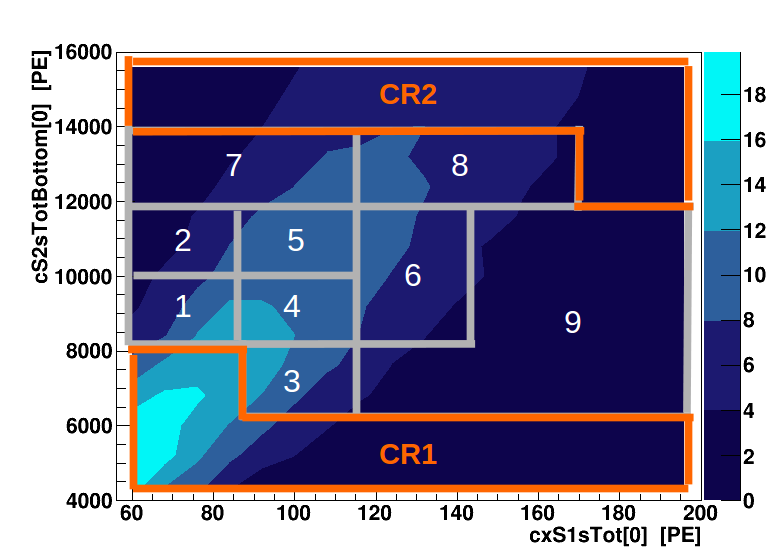
\includegraphics[width=\linewidth]{images/bkg_in_sr.png}
  \caption{Signal region and control region.}
  \label{fig:SR}
\end{figure}



\subsection{Signal Simulation} 
%description of the simulated signal, few words about cross checks MC matching.

The detector response to inelastic scattering of WIMPs  off $^{129}$Xe nucleus was simulated using an empirical model.
The total deposited energy is divided into two independent contributions: one related to the 39.6~keV de-excitation photon and the other  relative to
the simultaneous nuclear recoil of the xenon atom. The number of photons and charge yield detected is simulated separately for each contribution
and then added together.

The distribution in the cS1-cS2 plane of an ER induced by the de-excitation photon is simulated assuming a two dimensional normal pdf, $f(cS1,cS2)$, 
described except a normalization factor in equation~\ref{f:2dgaus}:
\begin{multline}
	f(cS1,cS2)  = exp \Big( -\frac{1}{2(1-\rho^2)} \Big[ \frac{(cS1 - \mu_{cS1})^2}{\sigma_{cs1}^2} + \\ 
	 \frac{(cS2 - \mu_{cS2})^2}{\sigma_{cs2}^2} - \frac{2\rho(cS1 - \mu_{cs1}) (cS2 - \mu_{cs2})} {\sigma_{cs1}\sigma_{cs2}} \Big] \Big) 
	%f(cS1,cS2) ~ = ~  \frac{1}{2 \pi \sigma_{cs1} \sigma_cs2 \sqrt{1-\rho^{2}} } exp \Big( -\frac{1}{2(1-\rho^2)} \Big[ \frac{(cS1 - \hat{cS1})^2}{\sigma_{cs1}^2} \Big] \Big)
\label{f:2dgaus}
\end{multline}
where $\mu_{cS1}$ and $\mu_{cS2}$ 
represents the average observed cS1 and cS2 given a 39.6~keVee , $\sigma_{cs1}$ and $\sigma_{cs2}$ are the standard deviation in cS1 and cS2 respectively,
while $\rho$ stands for the correlation between cS1 and cS2.
The detector related light yield $L_y$  at 39.6~keV, necessary to evaluate the average number of photon detected ($\mu_{cS1}$),
%with AmBe calibration has been found to have a large systematic uncertainty
%due to the contribution of the nuclear recoil, so the light yield used to describe the number of photon detected 
is obtained as the result of a NEST model~\cite{NEST,Geant1,Geant2} fit to data collected with several lines.  The same model is used to predict the charge yield at
39.6~keV which is then scaled according to the detector's secondary scintillation gain $Y$, determined from detector response to single electrons~\cite{SingleE}.
The detector resolution at 39.6~keV in cS1 and cS2 has been measured to be respectively 15.8\% and 14.7\% and used to extract the standard 
deviations $\sigma_{cs1}$, $\sigma_{cs2}$.  The correlation parameter is assumed to be independent of energy (at least in the considered range) and measured
using the 164~keV xenon activated line by $^{124}$AmBe calibration data, this line is chosen since allows to disentangle efficiently contribution from nuclear recoil.
The measured correlation is $\rho \, = \, -0.45 \pm 0.10$. 


The cS1 and cS2 distributions from NR contribution are predicted starting from the nuclear recoil energy spectrum
of WIMPs inelastic interaction~\cite{inelastic_th}. The average cS1 and cS2 are given by equations~\ref{f:cs1} and~\ref{f:cs2} respectively,
where $\mathcal{L}_{eff}$ is the liquid xenon NR relative scintillation efficiency, while $S_{ee} \, = \, 0.58$  and $S_{nr} \, = \, 0.95$ describe the scintillation 
quenching due to the electric field \cite{ScintQuenching}. The parameterization and uncertainties of $\mathcal{L}_{eff}$ as a function of $E_{nr}$ are based on existing 
direct measurements \cite{run8Result}. The light yield at 122~keVee originate from the same NEST model fit as described above. For the cS2 the parameterization 
of $Q_{Y}(E_{nr})$ is taken from \cite{QY}.
Finally all detector related resolution effects are introduced following the prescriptions described in \cite{dataAnalysis}.

\begin{equation}
cS1_{nr} ~=~ E_{nr} \, \mathcal{L}_{eff}(E_{nr}) \, L_{y} \, \frac{S_{nr}}{S_{ee}}
\label{f:cs1}
\end{equation}

\begin{equation}
cS2_{nr}  ~ = ~ E_{nr} \, Q_{Y}(E_{nr}) \, Y
\label{f:cs2}
\end{equation}

The pdf of the ER and NR contributions are then convoluted together to obtain the overall pdf of the signal.
%The two contribution are summed together in an event-by-event basis using random extraction from the two pdfs. 
A 2D (cS1 versus cS2) acceptance map is applied to the signal pdf to reproduce data selection effects. Acceptances are computed separately for each selection 
criteria using $^{124}$AmBe calibration sample, selections as the outer volume veto and the single scatter interaction represent an exception  and 
a dedicated computation has been performed in these cases. The selections acceptance average in the region of interest to about $0.80 \pm 0.05$. 
Figure~\ref{fig:SR} shows an example of full simulated signal model for a WIMP of 100~GeV mass. 

The signal simulation procedure has been validated reproducing the 39.6~keV xenon line from interaction due to
$^{124}$AmBe source and has been compared to data. For this comparison the proper  $^{124}$AmBe nuclear recoil and acceptances
were simulated. The simulated events were found in agreement  with calibration data within statistical uncertainties.

\begin{figure}[t!]
  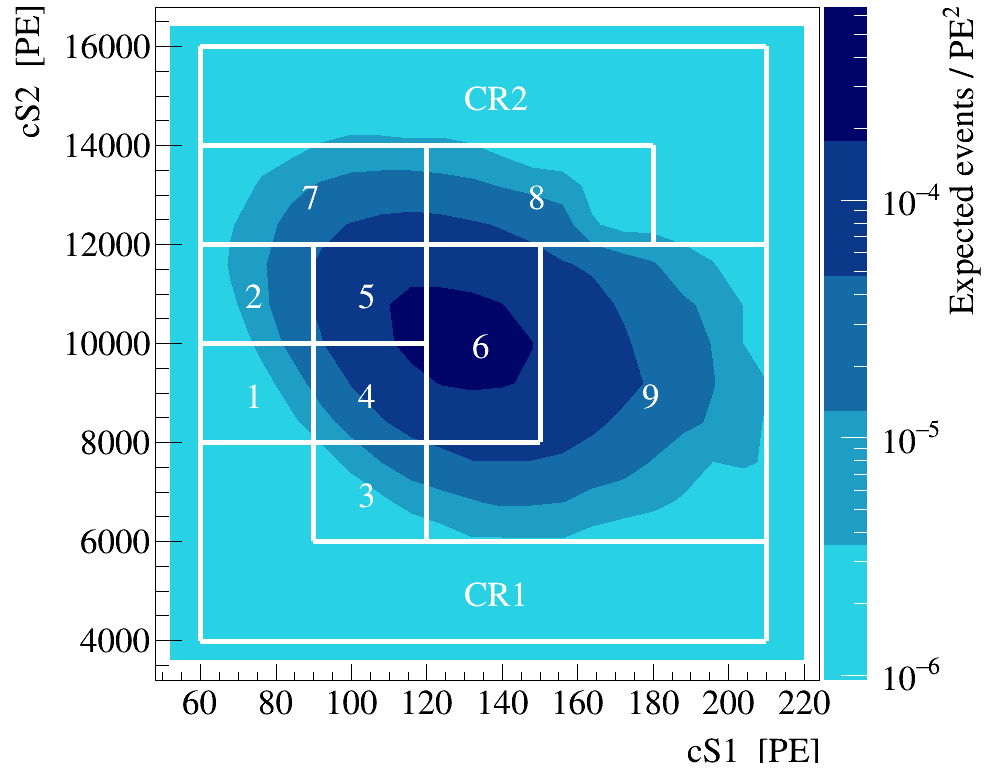
\includegraphics[width=\linewidth]{images/wimp_in_sr.png}
  \caption{Signal region and control region, for WIMP of mass 100~GeV.}
  \label{fig:SR2}
\end{figure}


\subsection {Background Model}

The main expected background contribution in the region of interest is due to eviromental and material radioactivity, its composition is mainly
represented by Compton scattering photons. Background contribution due to the activation of the xenon 39.6~keV line from radiogenic neutrons is expected to be negligible.

The background is modeled using data from the $^{60}$Co calibration campaign, which are assumed to well represent the background density distribution 
in the cS1-cS2 plane. 
The calibration sample yields  about 22'000 events in the ROI, these are then scaled to data according to a measured scale factor $\tau_{bkg}$.
This scale factor, which is merely the ratio between the data and calibration sample yields, is measured in the two control regions shown in Figure~\ref{fig:SR} and labelled CR1 and CR2. The two control 
regions give compatible results and the computed average is $\tau_{bkg} \, =  \, 0.034 \pm 0.002 $, where the reported uncertainty 
is of statistical nature only.

The distribution of the calibration sample has been compared to the data of the science run in the two control regions,
agreement is found within statistical uncertainties. Furthermore, $^{60}$Co calibration data have been compared in the region of interest to  
data from $^{232}$Th calibration campaign, the largest deviation between the two shapes is within 4\%. An additional systematic
uncertainty of 4\% has been applied to the expected background yield of each sub-region of the ROI.




\subsection{Systematic Uncertainties}

%FIXME: maybe change region definitions in order to have the sub-region 9 labelled as 7, so the signal would "nicely" look like a bump.
\begin{figure}[t!]
  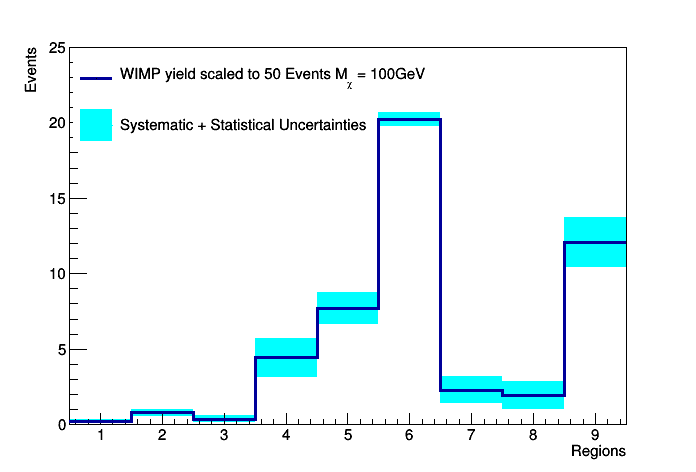
\includegraphics[width=\linewidth]{images/wimp_sys_unc.png}
  \caption{Signal region, uncertainties for WIMP of mass 100~GeV.}
  \label{fig:unc}
\end{figure}


Uncertainties on the total prediction of background events arise from the uncertainty on the measure of the normalization 
factor, $\tau_{bkg}$, and amount to 6\%, contribution of radiogenic neutrons are neglected. 
Systematic uncertainty on the shape of the predicted background distribution are assessed by the maximal discrepancy in the ROI between
the $^{60}$Co and $^{232}$Th calibration samples, a 4\% systematic additional to statistical uncertainty is assigned to the expected yield of each sub-region.
Note that uncertainties belonging to different sub-regions are considered independent from each other.
%It is important not only to describe correctly the expected total background but also its distribution

Uncertainty on the total yield of signal arising from selections acceptance uncertainties are found to be very weakly dependent on 
the WIMP mass, an overall 6\% acceptance uncertainty is then applied to all WIMPs hypothesis. 

Uncertainties on the energy scale and, more generally, related to detector response 
are parameterized using the respective uncertainties on the measure of $L_y$, $\mathcal{L}_{eff}$, $Y$, $Q_Y$ and $\rho$. The simulation shows 
that these type of uncertainties mainly affect the pdf of the signal model in the ROI, and very weakly the total signal yield. 
%For each WIMP mass we simulate several signal pseudo-sample, which are produced varying the model parameters  respectively of $\pm 1$ standard deviation. 
They are taken into account by simulating several signal pseudo-sample for each WIMP mass, the pseudo-samples are produced varying the model parameters respectively of $\pm 1$ standard deviation. 
For each sub-region is then computed an overall uncertainty by adding in quadrature the variations of each pseudo-sample 
%FIXME: explain this better, the up variation are separated from down variations and added together
with respect to nominal. Figure~\ref{fig:unc} is an example of such a systematic uncertainty computation for a WIMP of 100~GeV mass.


%FIXME: express this in an understandable way
All the uncertainties discussed here are parameterized within a binned profiled likelihood function using the framework~\cite{roostat,roofit}.
All parameters related to systematic uncertainties are assumed to be normally distributed.


















